% ---------------------------------------------------------------------------
% Member 1 section: Kolipakula Sai Tushaar - what students do.
% DONE - no edits needed. Every number below is produced by
% Member1/m1_clustering_workflow.py and stored in Member1/outputs/m1_results.json.
% ---------------------------------------------------------------------------
\section{Kolipakula Sai Tushaar: Habit Profiles (Clustering)}
\label{sec:m1}

\paragraph{Driving question.} A1 (Appendix, Figs.~1--11) showed that study hours, sleep,
exercise and the leisure share of screen time each move the exam score by a few
points. A3 asks the next question: \emph{do students form distinct habit
profiles, and does belonging to a ``good-habits'' profile give an exam
advantage beyond the student's prior attainment?} Clustering is the right tool
because it groups students by their whole habit pattern without being told the
outcome; the outcome is only used afterwards to judge the groups.

\paragraph{Method summary.} K-means~\cite{lloyd1982} on standardised features
(scaler fitted on the training split, scikit-learn~\cite{pedregosa2011}), with the number of clusters $k$ chosen from four
diagnostics: the elbow in inertia, the silhouette~\cite{rousseeuw1987} compared against a
\emph{shuffled null} (each column permuted independently, which keeps every
variable's distribution but destroys any joint structure), seed stability
(mean adjusted Rand index~\cite{hubert1985} between six single-start runs) and Gaussian-mixture
BIC. The Hopkins statistic~\cite{hopkins1954} is reported as a supporting check.
Cluster differences in score are tested with Kruskal--Wallis~\cite{kruskal1952} and
$\eta^2_H$ (iteration~1), and with Welch's $t$~\cite{welch1947}, Mann--Whitney
$U$~\cite{mann1947}, Cohen's $d$~\cite{cohen1988} and 1{,}000-sample bootstrap
confidence intervals~\cite{efron1993} (iteration~2). A gradient-boosting
regressor~\cite{friedman2001} with permutation importance~\cite{breiman2001}
cross-checks the clustering result. Iteration~2 is
confirmed on the 16{,}000-student test split, which no model or adjustment
ever saw. Fig.~\ref{fig:m1-workflow} shows the full workflow.

\begin{sidewaysfigure}
  \centering
  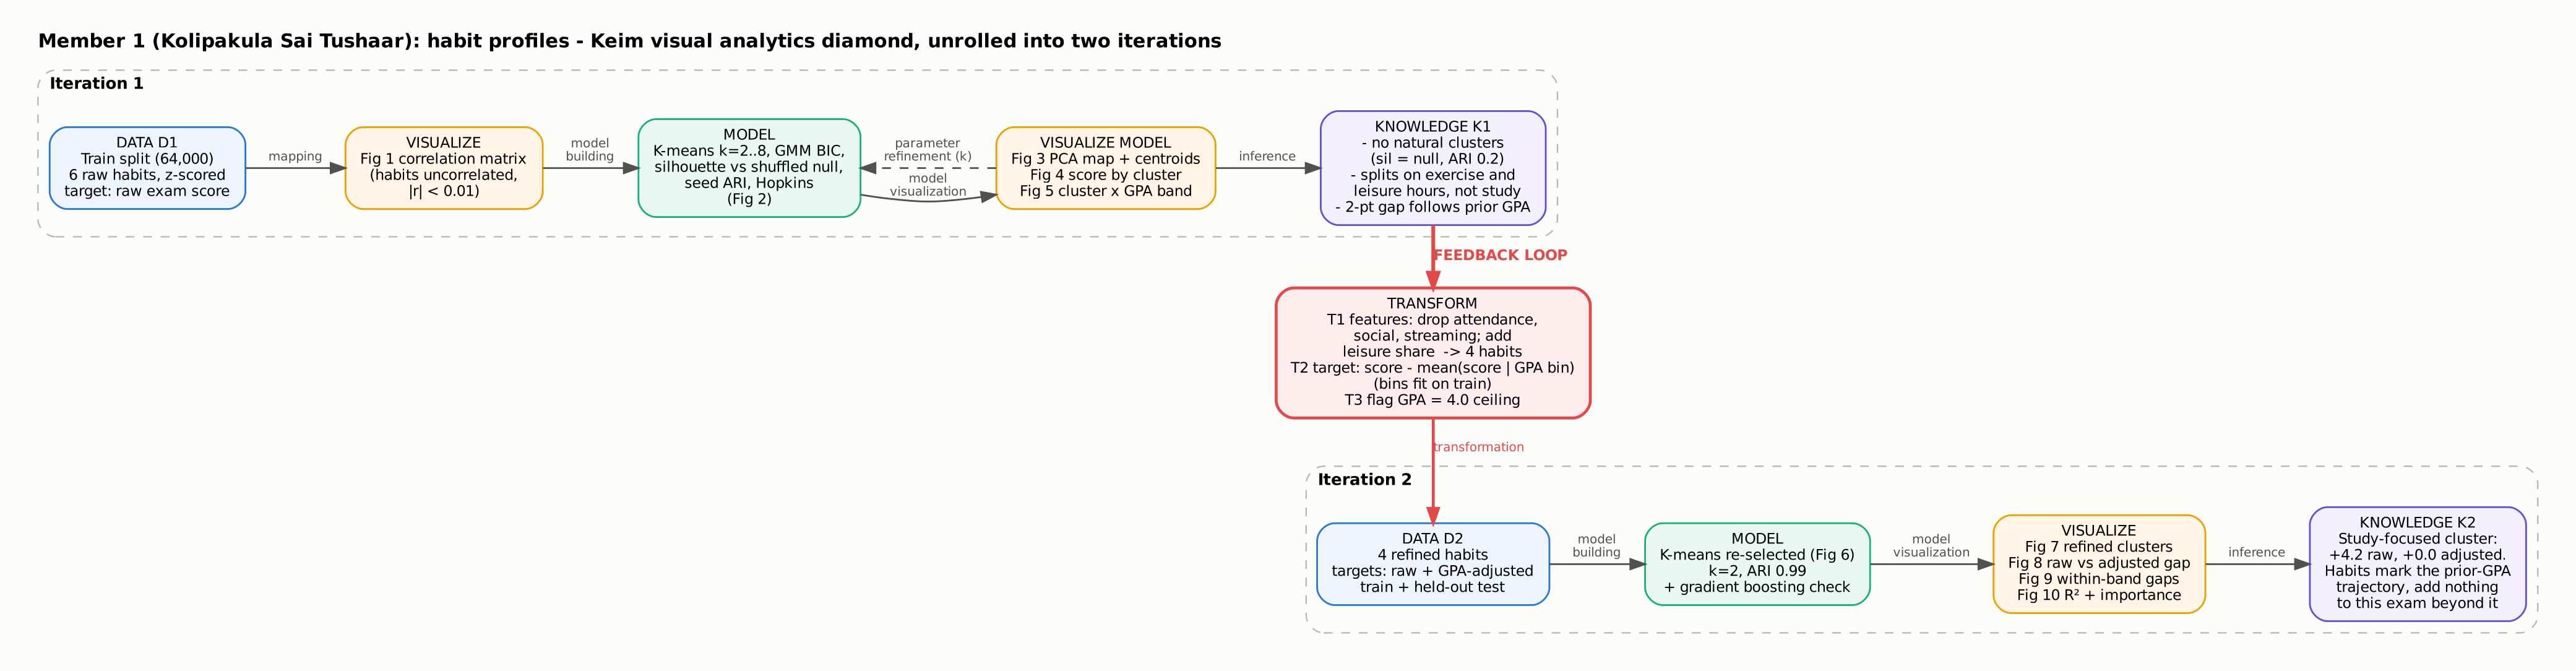
\includegraphics[width=\textheight]{images/M1_workflow_unrolled.png}
  \caption{Member~1's workflow as the Keim et~al.\ diamond unrolled into two
  iterations. The only self-loop is the parameter refinement of $k$ inside
  iteration~1. The edge labelled \emph{Feedback loop} carries the iteration-1
  inference into three data transformations (T1--T3) that define the data for
  iteration~2.}
  \label{fig:m1-workflow}
\end{sidewaysfigure}

\begin{table}[htbp]
  \centering\small
  \caption{Task sequence and the reason behind each visualization.}
  \label{tab:m1-tasks}
  \begin{tabular}{@{}lllp{10.4cm}@{}}
    \toprule
    Stage & Fig. & Task & Why this chart \\
    \midrule
    V1 & \ref{fig:m1-corr} & Correlate & A matrix shows every pair at once; any joint structure clustering could find must show up here first. \\
    M1 & \ref{fig:m1-k1} & Select $k$ & Four small multiples on one $k$ axis; the dashed null line makes ``better than random'' visible. \\
    V1 & \ref{fig:m1-map1} & Overview & Hexbin density (80k points would overplot); clusters faceted, not overlaid, because four hues on one scatter are not colour-blind safe. Heatmap gives the profile. \\
    V1 & \ref{fig:m1-score1} & Compare & Violins show the overlap; means with CIs show the size of the gap on a readable scale. \\
    V1 & \ref{fig:m1-conf1} & Explain & 100\% stacked bars for composition; dot plot within each band to test the confound. \\
    M2 & \ref{fig:m1-k2} & Re-select $k$ & Same panels as Fig.~\ref{fig:m1-k1} with D1 in grey, so the change is the only new information. \\
    V2 & \ref{fig:m1-map2} & Overview & With two clusters a direct scatter is legible; diverging bars give centroids in $z$ with raw-unit labels. \\
    V2 & \ref{fig:m1-gap} & Compare & One axis (points) for raw, adjusted and GPA gaps, so the reader compares lengths directly. \\
    V2 & \ref{fig:m1-band} & Search & Raw and adjusted gap side by side per band locates where any gap survives. \\
    M2/V2 & \ref{fig:m1-sup} & Validate & A supervised model confirms the clustering conclusion with a different method. \\
    \bottomrule
  \end{tabular}
\end{table}

% ---------------------------------------------------------------------------
\subsection{Iteration 1: clustering the six raw habits}

\paragraph{Data D1.} Six raw, non-derived habit variables from the training
split: daily study hours, sleep hours, weekly exercise, attendance, social
media hours and streaming hours. Derived columns are left out so that no
behaviour is counted twice.

\begin{figure}[htbp]
  \centering
  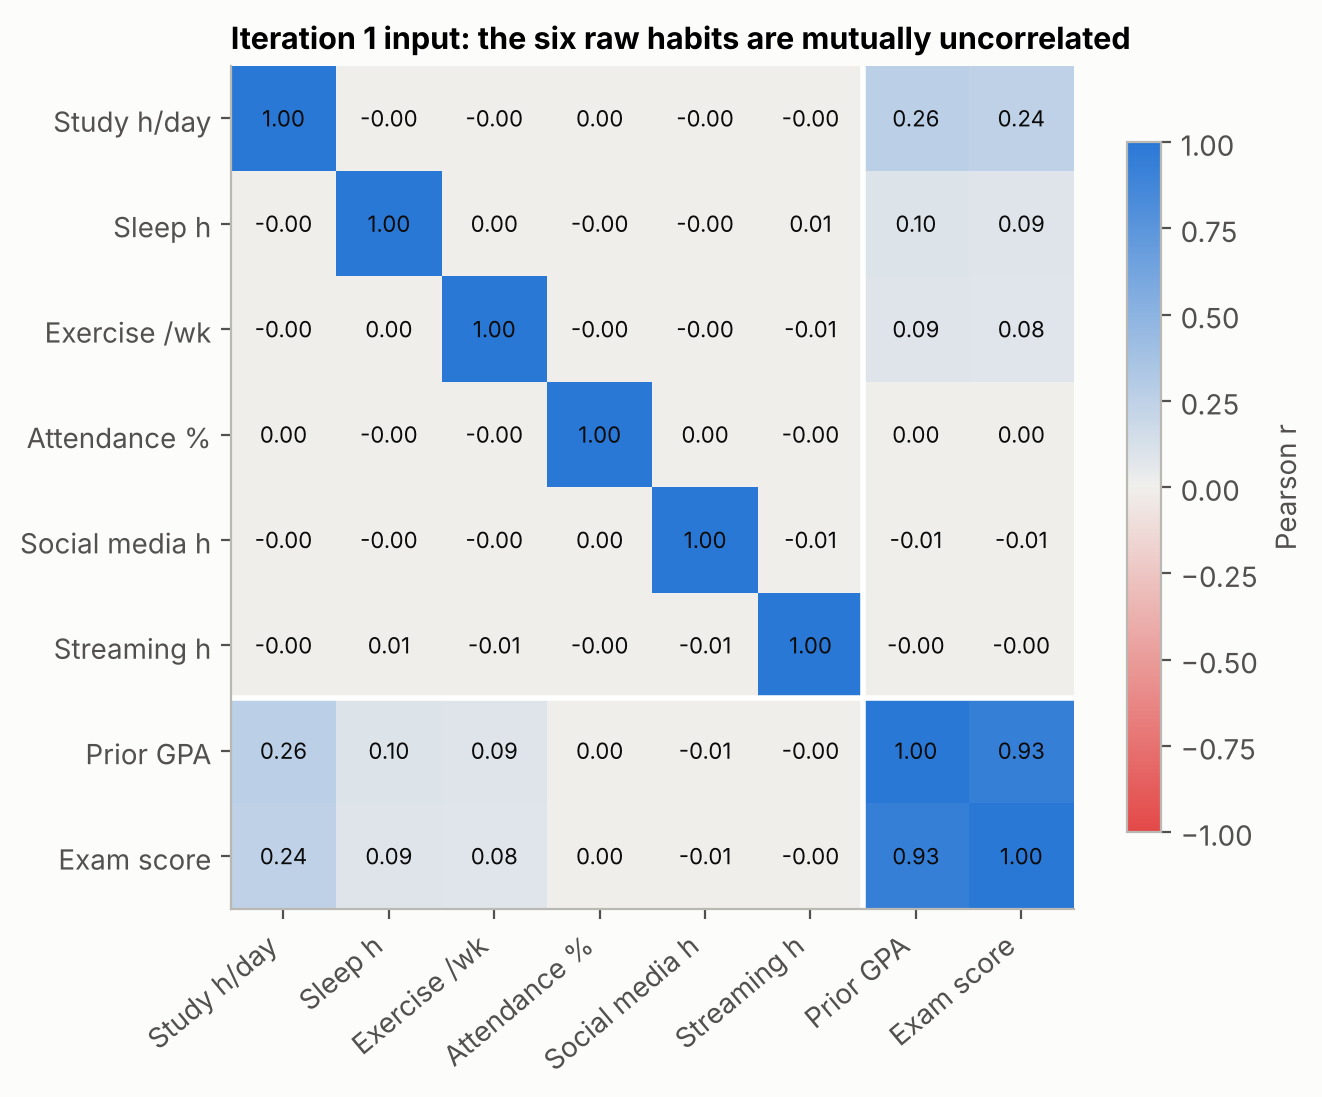
\includegraphics[width=0.62\textwidth]{images/M1_fig01_habit_correlations.png}
  \caption{Pearson correlations among the six habits, prior GPA and exam score
  (training split). Off the diagonal, no pair of habits correlates above
  $|r|=0.007$. Only study hours ($r=0.24$), sleep (0.09) and exercise (0.09)
  relate to the exam score, and each relates almost equally to prior GPA.}
  \label{fig:m1-corr}
\end{figure}

Fig.~\ref{fig:m1-corr} is the first warning. The six habits are statistically
independent of each other, so the habit space has no obvious joint structure
for clustering to find. Attendance, social media and streaming hours have no
correlation with the score at all ($|r|\le 0.006$).

\begin{figure}[htbp]
  \centering
  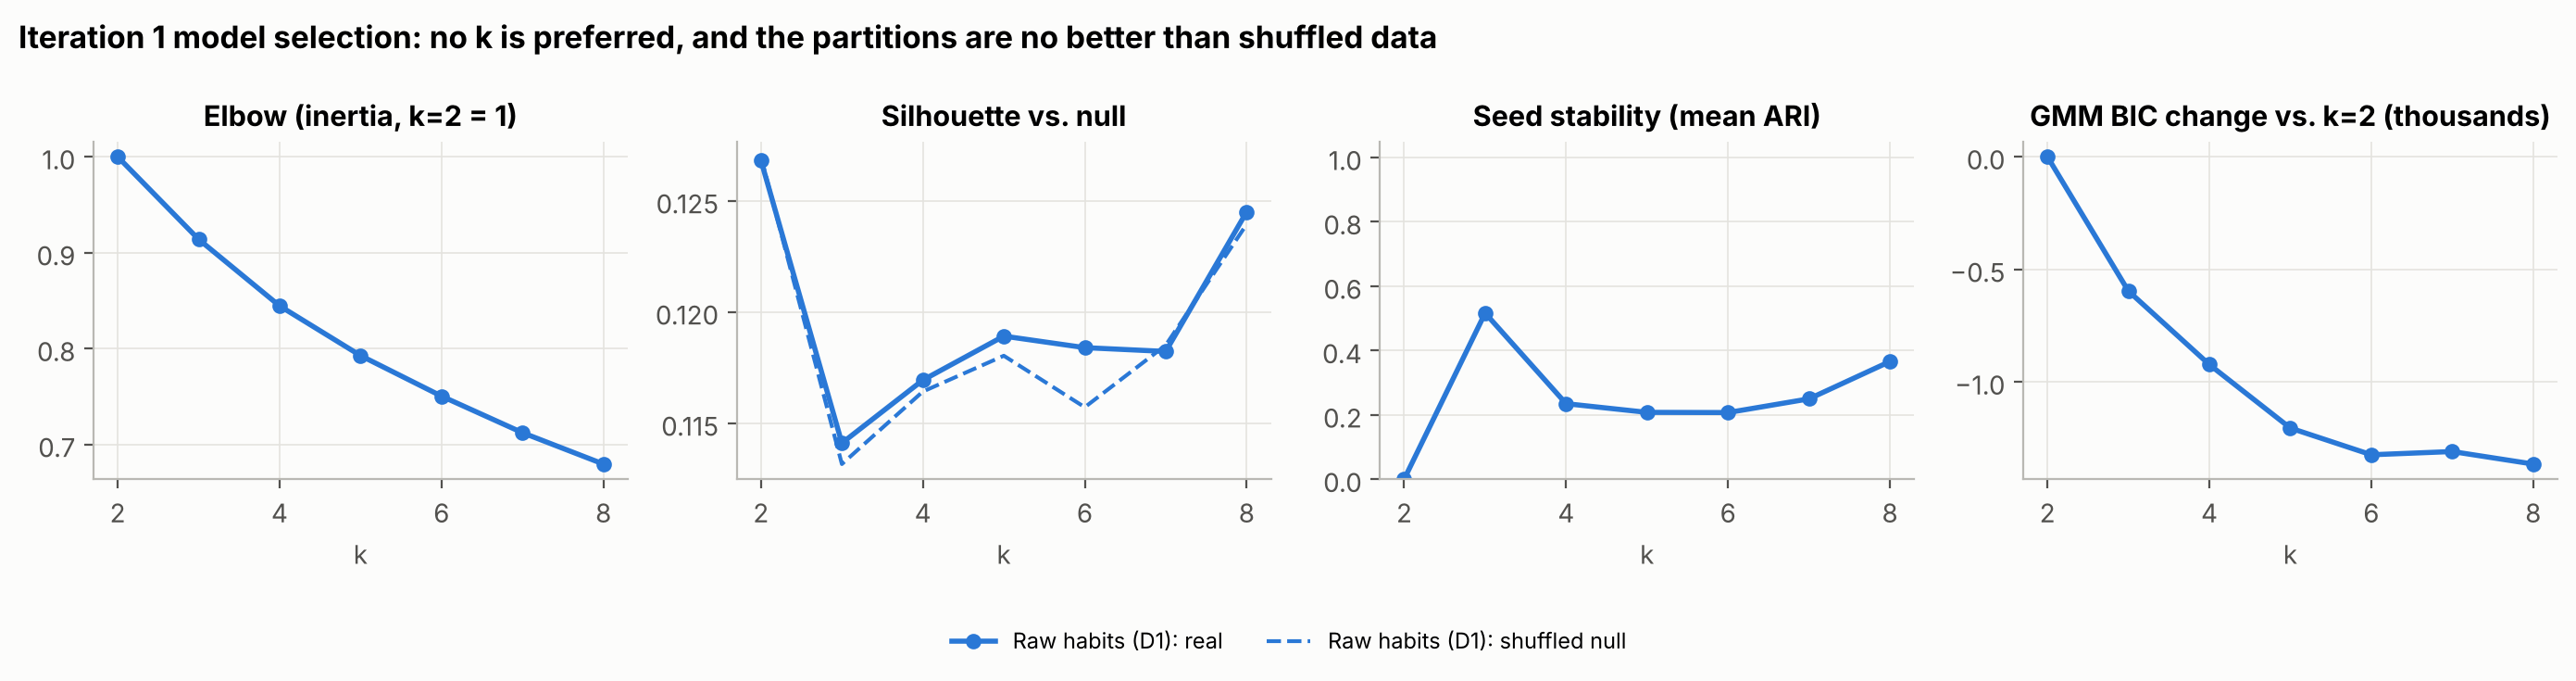
\includegraphics[width=\textwidth]{images/M1_fig02_k_selection_raw.png}
  \caption{Choosing $k$ on D1. The elbow is smooth, GMM BIC keeps falling, the
  real silhouette (solid) lies on top of the shuffled null (dashed) at every
  $k$, and seed stability never exceeds ARI 0.52. No $k$ is preferred.}
  \label{fig:m1-k1}
\end{figure}

\paragraph{Model M1.} Fig.~\ref{fig:m1-k1} shows that K-means finds nothing
the shuffled data does not also produce: at $k=4$ the silhouette is 0.117
against 0.116 for the null, and two runs with different seeds agree only at
ARI 0.24. At $k=2$ the ARI is 0.00, because a round cloud can be cut in half
along any direction. The Hopkins statistic is 0.61, only slightly above the
0.5 expected for random data; the excess comes from the non-uniform shapes of
the individual variables, which the shuffled null keeps. Since every criterion is flat, $k=4$ was kept for
readable profiles. The choice of $k$ is arbitrary, and that is part of the
finding.

\begin{figure}[htbp]
  \centering
  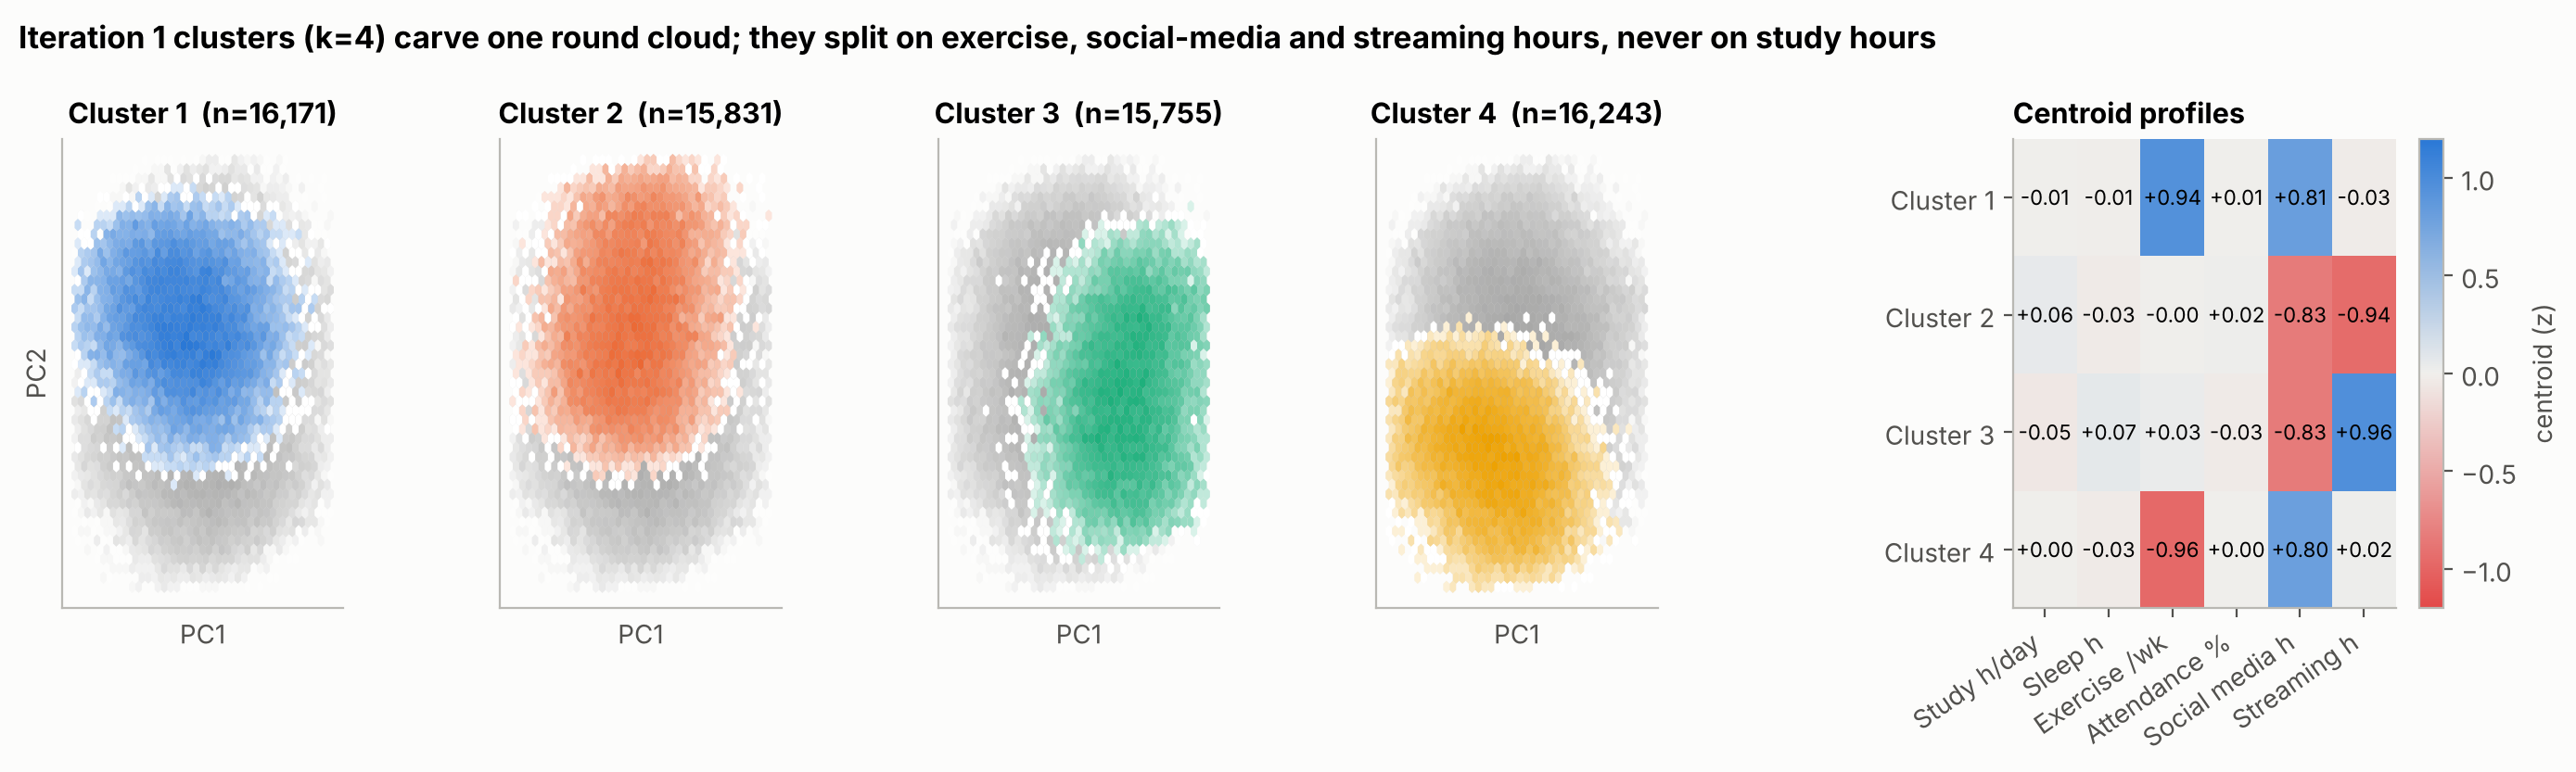
\includegraphics[width=\textwidth]{images/M1_fig03_cluster_map_raw.png}
  \caption{Iteration-1 clusters ($k=4$) on the first two principal components
  (which explain only 16.9\% and 16.7\% of variance). Each panel shows one
  cluster over the grey density of all students. The heatmap gives centroids in
  $z$-units: clusters differ by up to 1.9\,SD in exercise and streaming and
  1.6\,SD in social media, but by only 0.1\,SD in study hours and sleep.}
  \label{fig:m1-map1}
\end{figure}

Fig.~\ref{fig:m1-map1} shows K-means slicing one round cloud into four wedges.
The slices are defined by exercise, social media and streaming hours, two of
which have no relation to the score. Study hours, the habit most related to
the score, does not separate the clusters at all.

\begin{figure}[htbp]
  \centering
  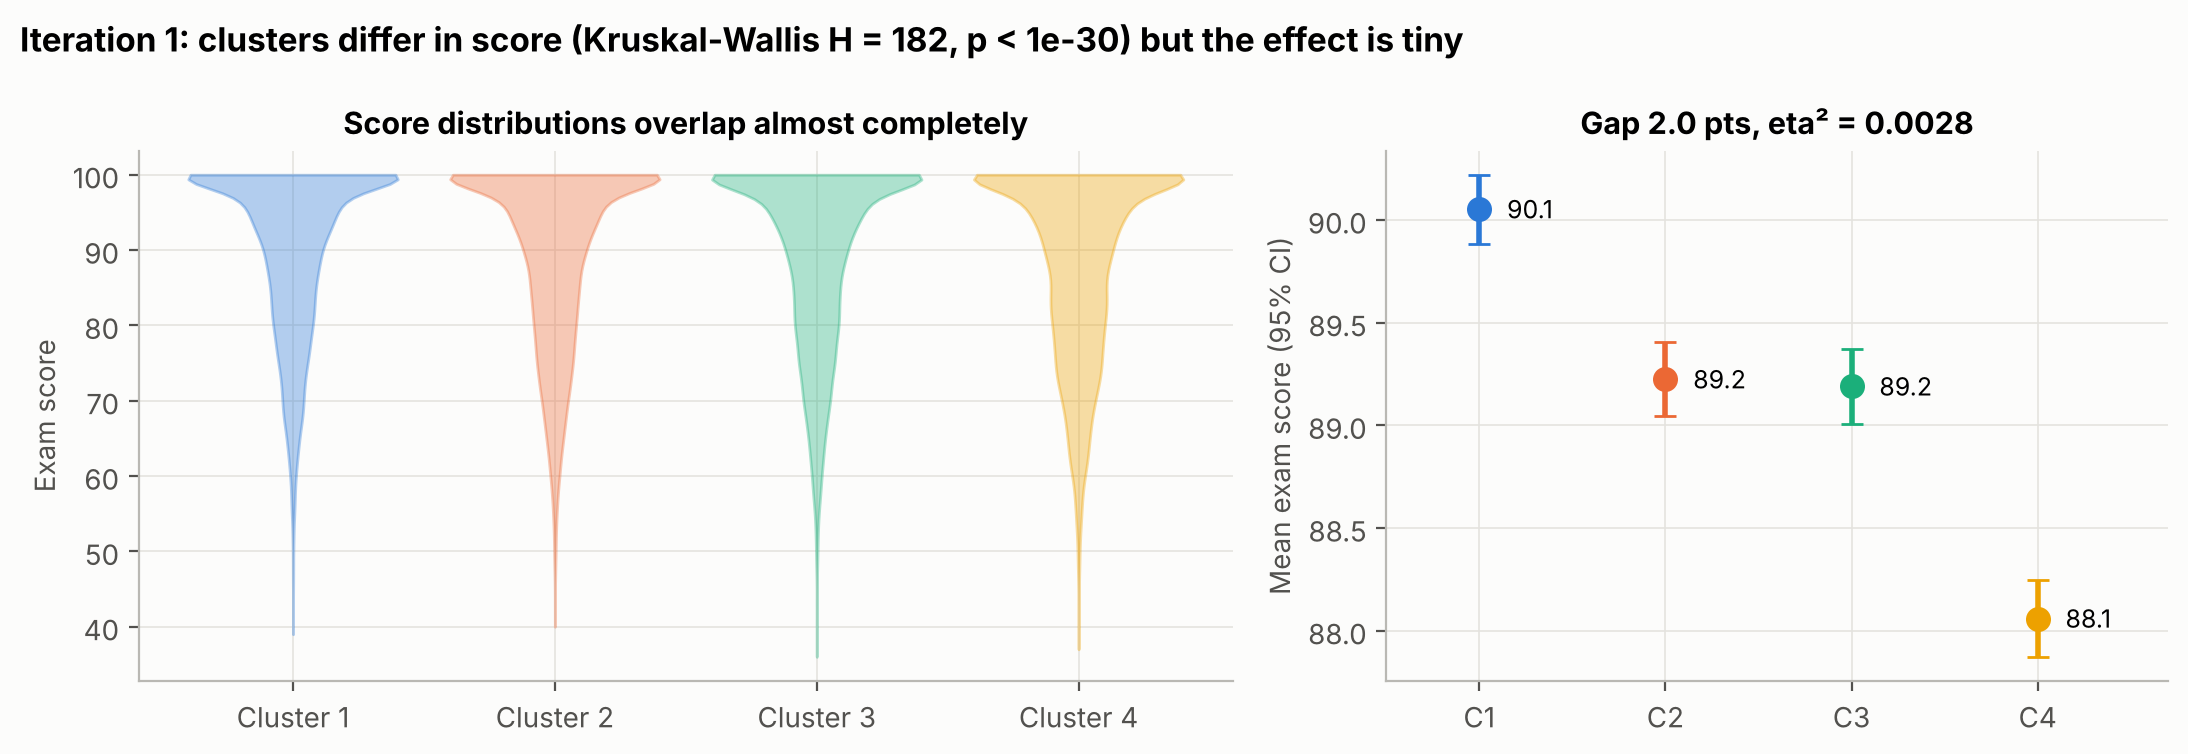
\includegraphics[width=\textwidth]{images/M1_fig04_score_by_cluster_raw.png}
  \caption{Exam score by iteration-1 cluster. The difference is statistically
  significant (Kruskal--Wallis $H=182$, $p=3\times10^{-39}$) but the effect
  size is negligible ($\eta^2_H=0.0028$): the best and worst clusters differ by
  2.0 points (90.1 vs.\ 88.1), and the distributions overlap almost entirely.}
  \label{fig:m1-score1}
\end{figure}

\begin{figure}[htbp]
  \centering
  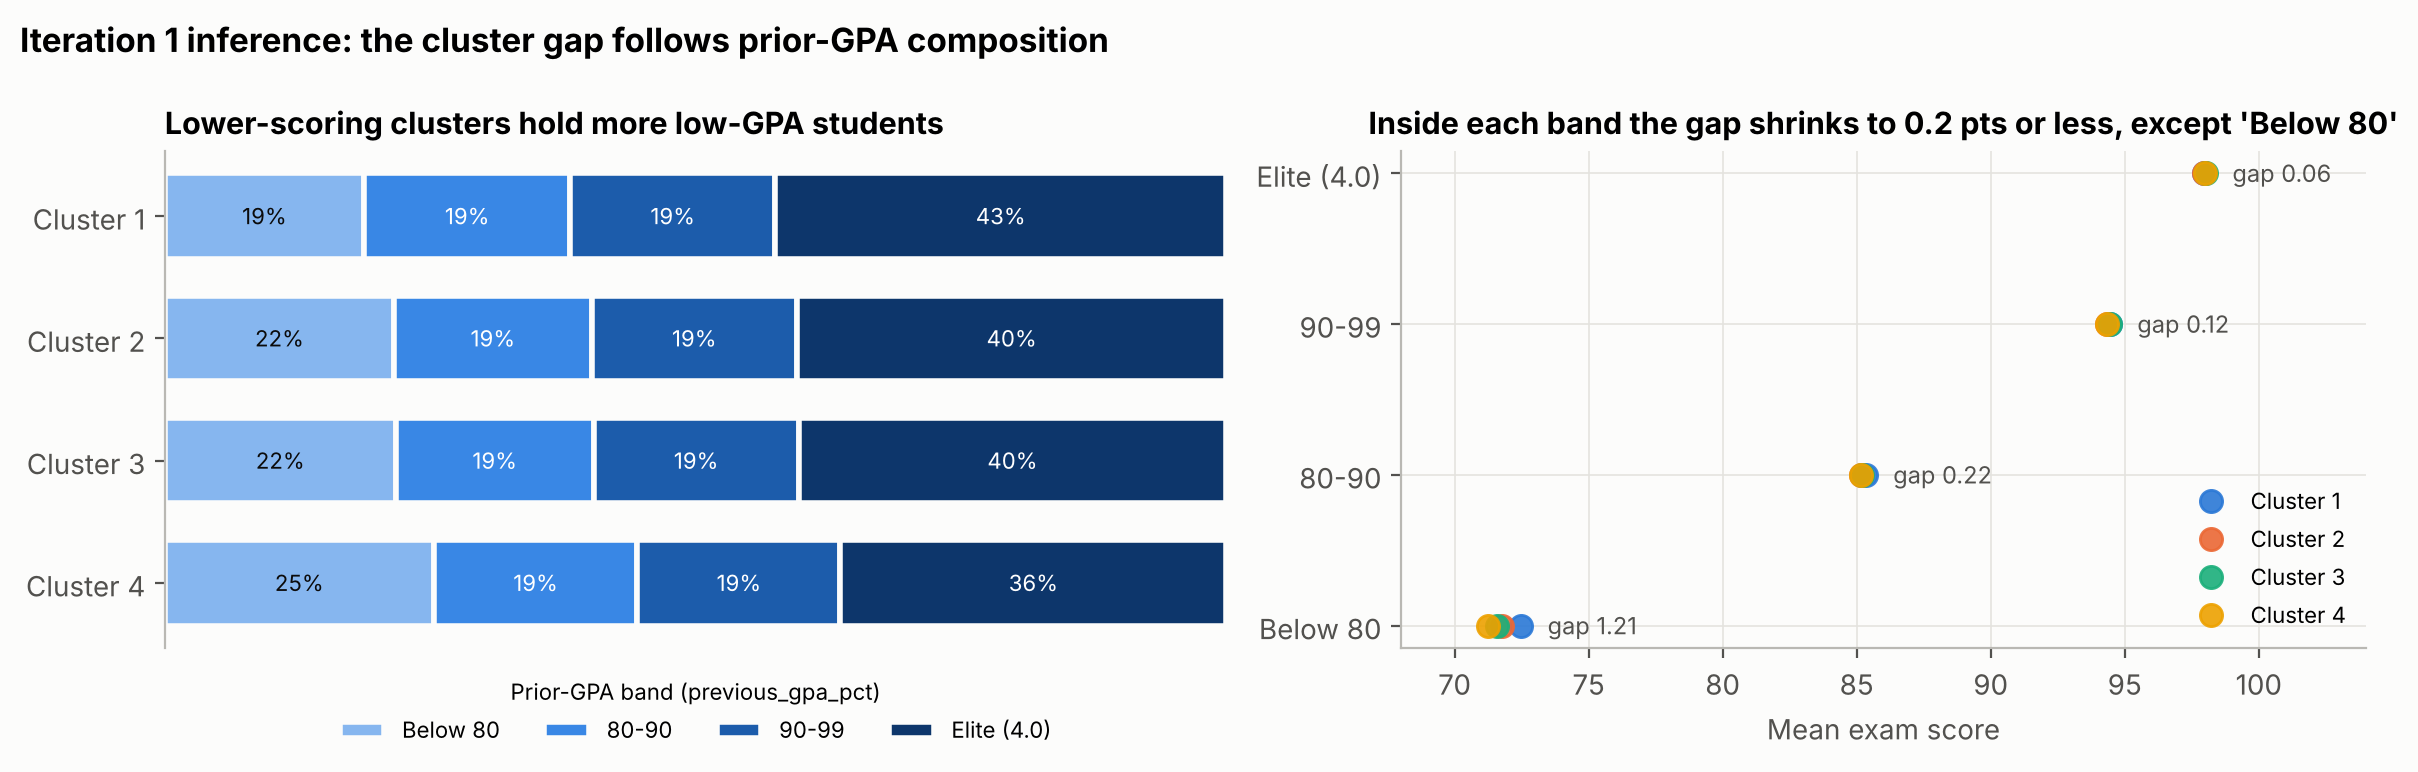
\includegraphics[width=\textwidth]{images/M1_fig05_gpa_confound_raw.png}
  \caption{Left: share of each cluster in each prior-GPA band. The lowest
  scoring cluster (C4) holds 25.3\% Below-80 students against 18.8\% for the
  highest (C1). Right: mean score per cluster inside each band. The cluster
  gap shrinks from 2.0 points to 0.06--0.22 points in the upper three bands;
  1.2 points remain in the Below-80 band.}
  \label{fig:m1-conf1}
\end{figure}

\paragraph{Knowledge K1.} Figs.~\ref{fig:m1-score1} and~\ref{fig:m1-conf1}
lead to three inferences:
\begin{enumerate}
  \item \textbf{The raw habit space has no natural clusters.} The silhouette
        equals that of shuffled data and partitions change with the random
        seed, so the iteration-1 clusters are arbitrary slices, not student
        types.
  \item \textbf{The slices follow the wrong variables.} Because the six
        habits are independent and equally weighted after scaling, K-means
        splits on whichever axes it happens to pick: here exercise, social
        media and streaming, not study hours. Raw leisure hours carry no signal;
        A1 (Appendix, Fig.~8) showed that the \emph{share} of screen time spent on
        leisure is what relates to performance.
  \item \textbf{The small score gap that exists is mostly prior GPA.} The
        clusters differ in their mix of prior-GPA bands, and inside a band the
        gap nearly disappears. The 1.2 points left in the Below-80 band need
        explaining: that band spans GPA 1.64--3.20, so students in it still
        differ a lot in prior attainment.
\end{enumerate}

% ---------------------------------------------------------------------------
\subsection{Feedback loop: transforming the data}

Each inference maps to one transformation of the data:

\begin{description}
  \item[T1 (feature space, from inferences 1--2).] Drop attendance, social media
        hours and streaming hours; add \texttt{leisure\_screen\_share}. The new
        space D2 holds four habits: study hours, sleep, exercise and leisure
        share. Leisure share correlates $r=-0.64$ with study hours, partly by
        construction (screen time includes study time). This dependence is
        what gives the space a real axis to cluster on: study-dominant versus
        leisure-dominant screen use.
  \item[T2 (target, from inference 3).] Replace the raw score with a
        \emph{GPA-adjusted score}: the student's score minus the mean score of
        all training students in the same prior-GPA bin (24 bins 0.1 GPA wide
        below 4.0, plus GPA exactly 4.0 as a 25th bin). Bin means are learned on the
        training split only and applied unchanged to the test split. These bin
        means alone explain $R^2=0.870$ of test-set score variance, so the
        adjusted score is the part of the exam that prior GPA does not predict
        (SD 4.2 points). Binning, rather than a straight-line fit, follows the
        curve near the ceiling without assuming its shape.
  \item[T3 (censoring).] 39.9\% of training students have GPA 4.0, and 53.6\%
        of those score exactly 100, so their adjusted score is capped. Every
        iteration-2 result is repeated with these students excluded.
\end{description}

% ---------------------------------------------------------------------------
\subsection{Iteration 2: clustering the refined habits}

\begin{figure}[htbp]
  \centering
  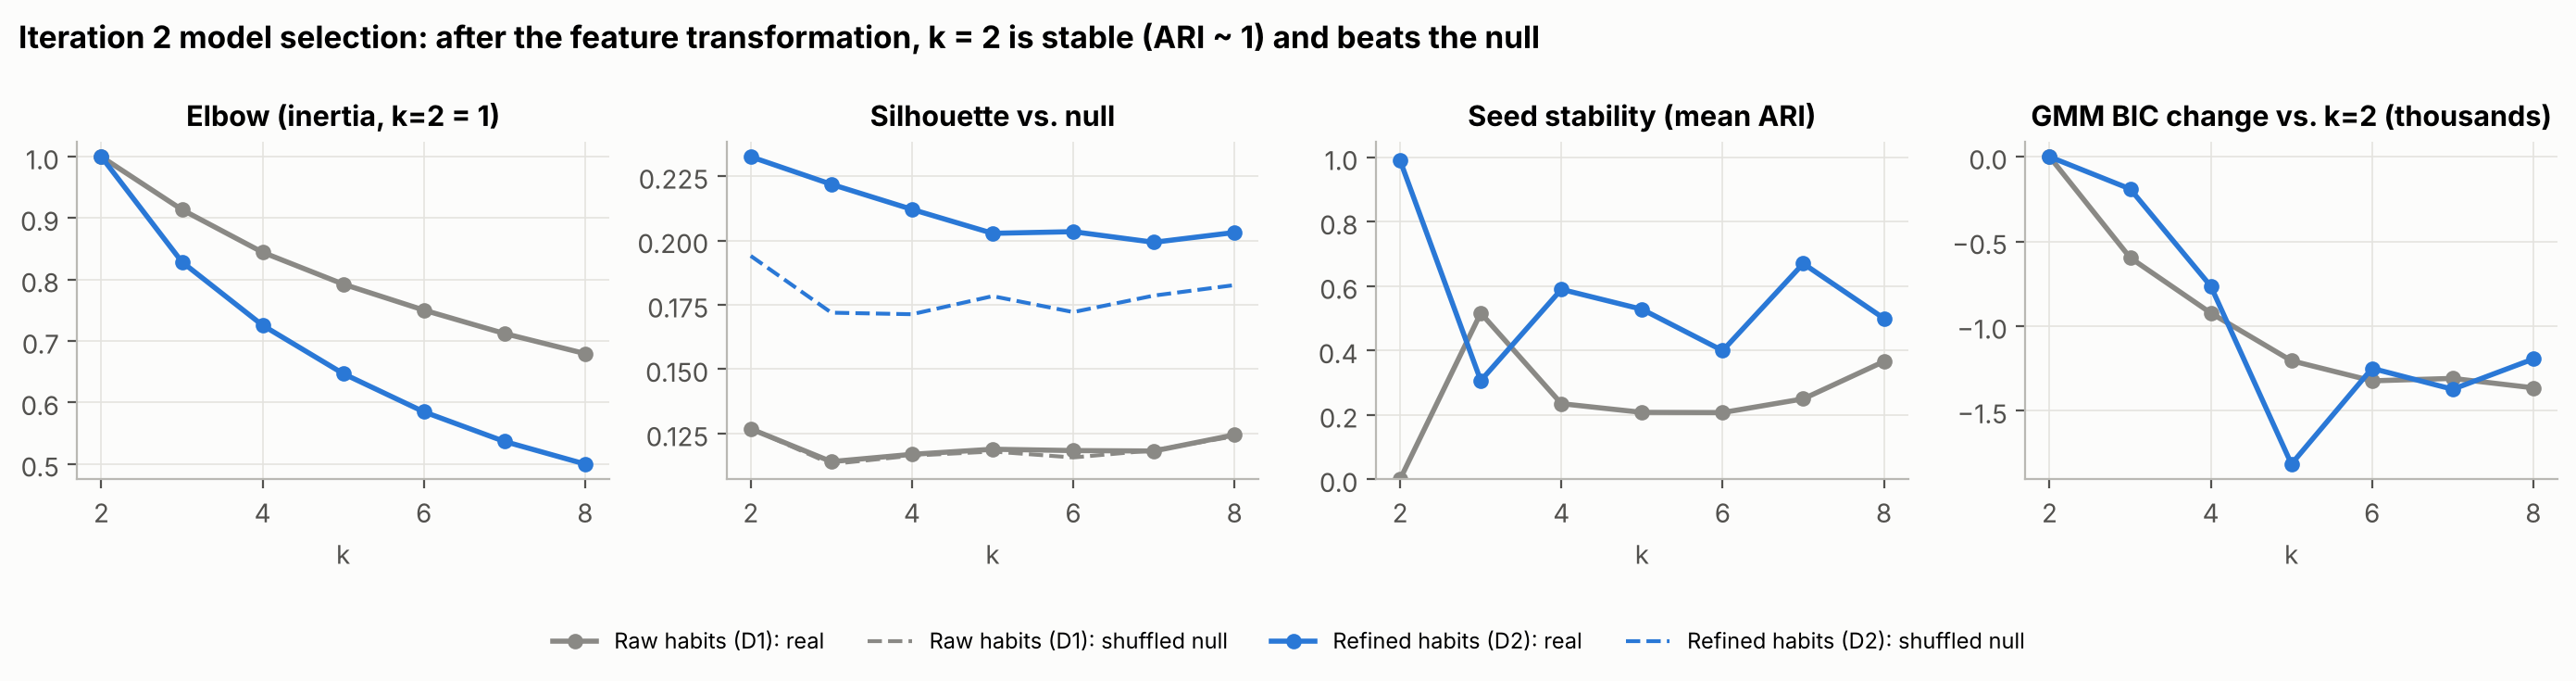
\includegraphics[width=\textwidth]{images/M1_fig06_k_selection_refined.png}
  \caption{Choosing $k$ on D2 (blue) against D1 (grey). At $k=2$ the refined
  space is now stable (ARI 0.99) and clearly above its null (silhouette 0.233
  vs.\ 0.194). GMM BIC is lowest at $k=5$, but that solution is not stable
  (ARI 0.53), so $k=2$ is used.}
  \label{fig:m1-k2}
\end{figure}

\paragraph{Model M2.} After T1, Fig.~\ref{fig:m1-k2} shows a real, repeatable
structure: six runs agree almost perfectly at $k=2$, and the silhouette beats
the shuffled null at every $k$. The pipeline selects $k$ automatically as the
most stable value. The Hopkins statistic rises to 0.88, but it is not used to
choose $k$: the leisure share and study hours fill only a triangular region
(Fig.~\ref{fig:m1-map2}), and a uniform reference sample drawn over the
bounding box inflates the statistic.

\begin{figure}[htbp]
  \centering
  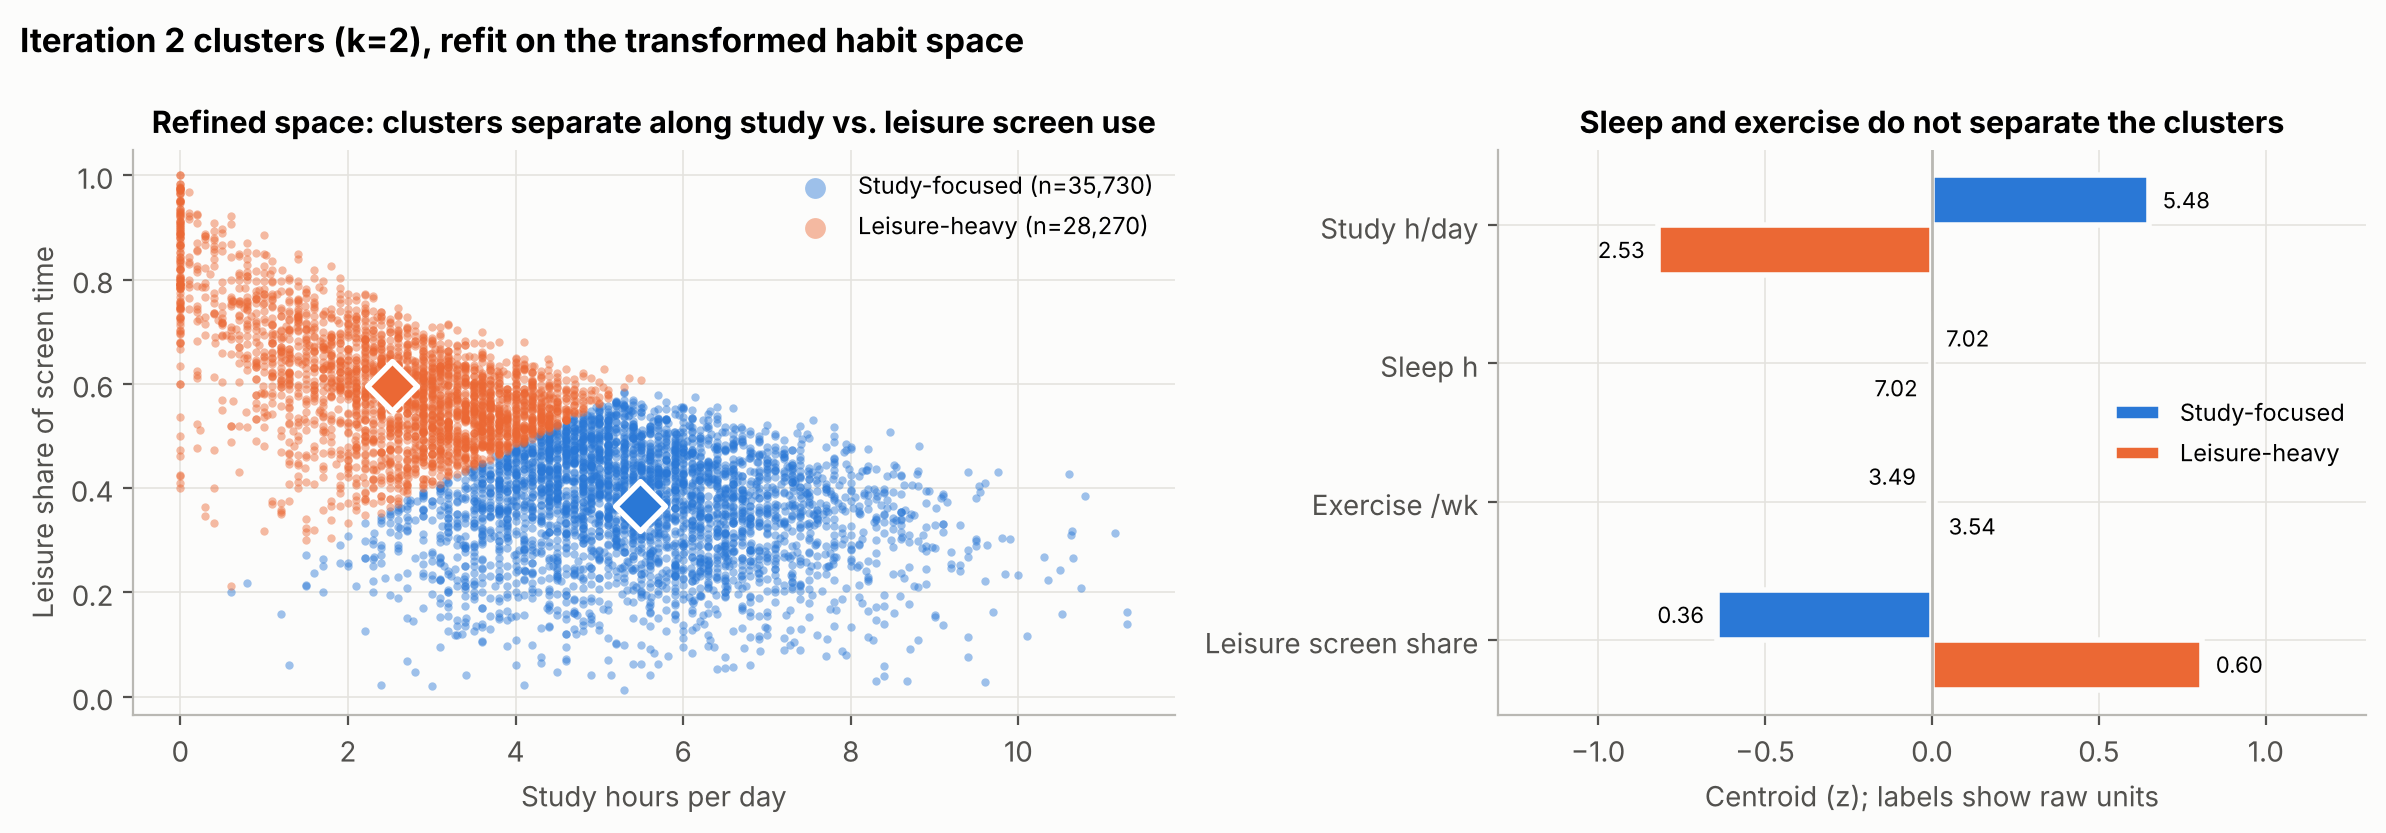
\includegraphics[width=\textwidth]{images/M1_fig07_cluster_map_refined.png}
  \caption{The two refined clusters. \emph{Study-focused} (35{,}730 training
  students) studies 5.5\,h/day with 37\% of screen time on leisure;
  \emph{Leisure-heavy} (28{,}270) studies 2.5\,h/day with 60\% on leisure.
  Sleep (7.0\,h both) and exercise (3.5 vs.\ 3.5 days) do not differ.
  Diamonds mark centroids.}
  \label{fig:m1-map2}
\end{figure}

\begin{figure}[htbp]
  \centering
  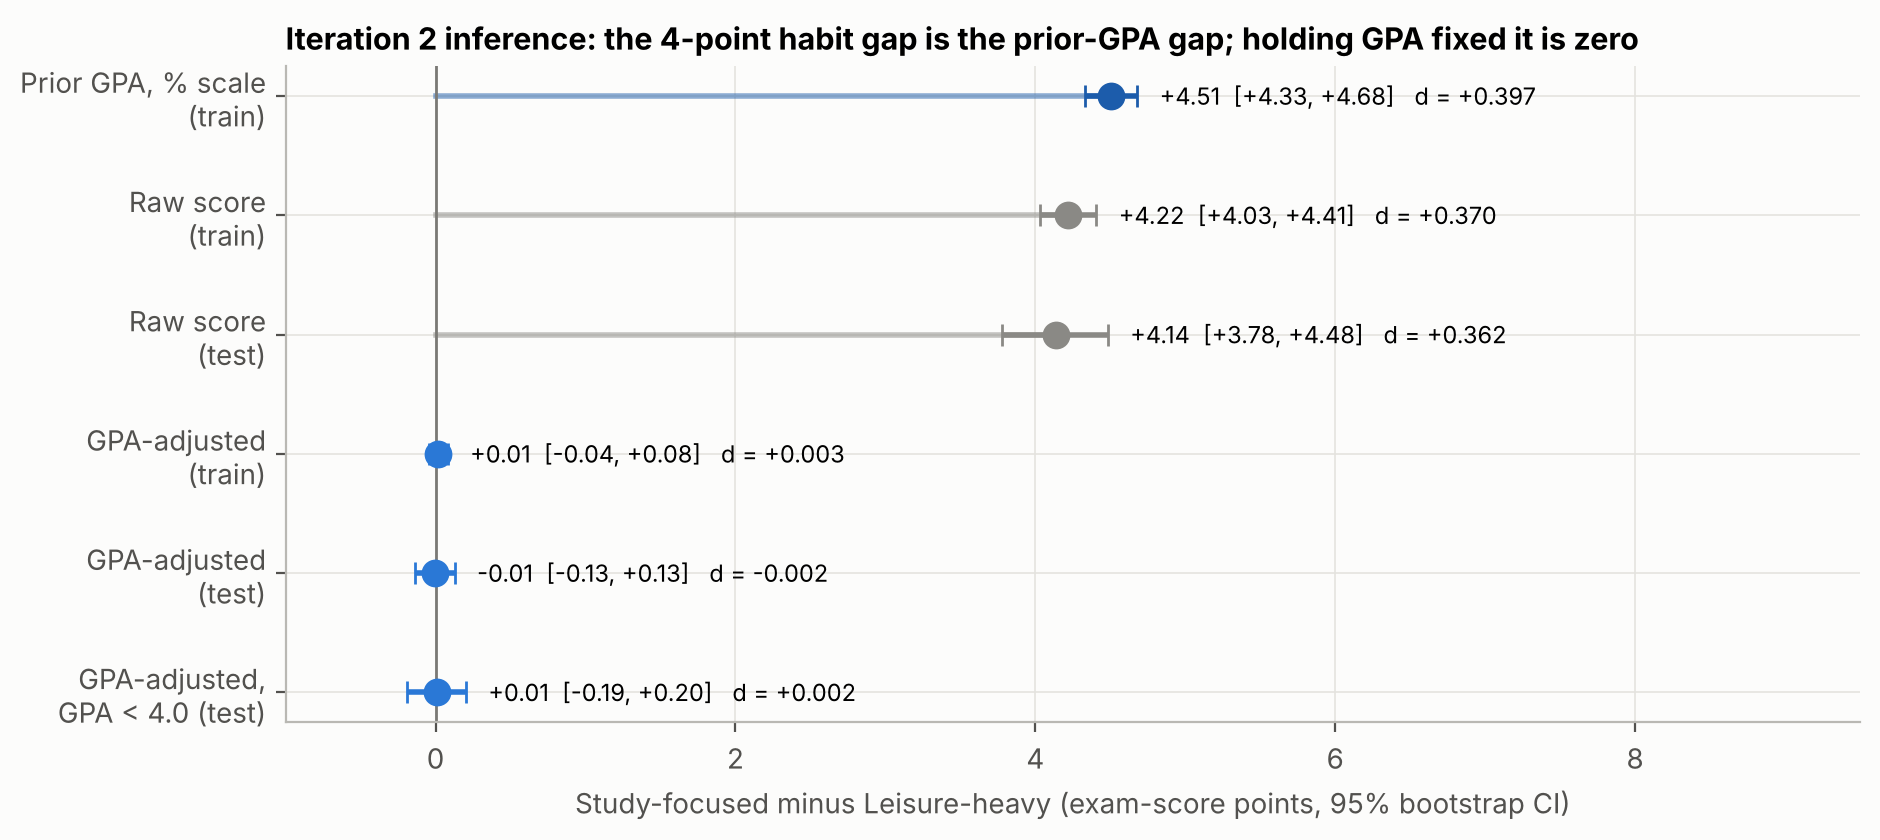
\includegraphics[width=\textwidth]{images/M1_fig08_raw_vs_adjusted_gap.png}
  \caption{Study-focused minus Leisure-heavy, in exam-score points, with 95\%
  bootstrap CIs. The raw gap is 4.2 points (test 4.1, $d=0.36$). The same
  clusters differ by 4.5 points in prior GPA on the percentage scale. On the
  GPA-adjusted score the gap is $+0.01$ (train) and $-0.01$ (test, CI
  $-0.13$ to $+0.13$, Welch $p=0.92$, $d=-0.002$), and stays at $+0.01$ with
  GPA-4.0 students removed.}
  \label{fig:m1-gap}
\end{figure}

\begin{figure}[htbp]
  \centering
  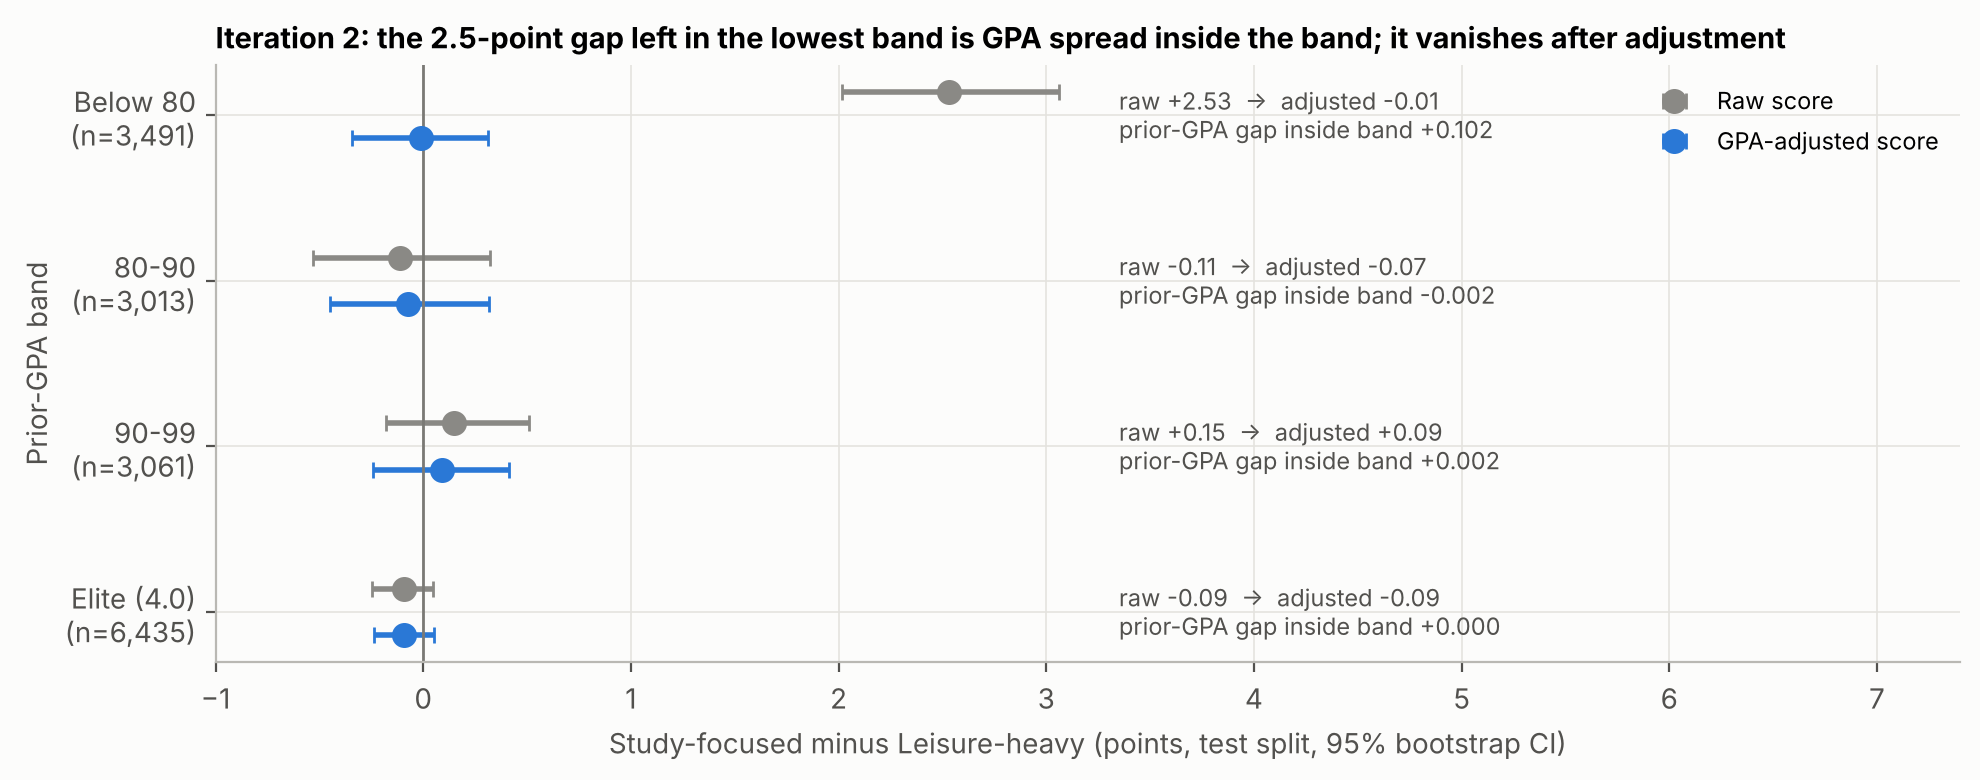
\includegraphics[width=\textwidth]{images/M1_fig09_within_band_refined.png}
  \caption{Gap per prior-GPA band on the test split, raw (grey) and adjusted
  (blue). The only raw gap left, 2.5 points in the Below-80 band, matches a
  0.10-point GPA difference between the clusters \emph{inside} that band. After
  adjustment it is $-0.01$ (CI $-0.34$ to $+0.31$). In the other bands both
  gaps are within $\pm0.15$.}
  \label{fig:m1-band}
\end{figure}

\begin{figure}[htbp]
  \centering
  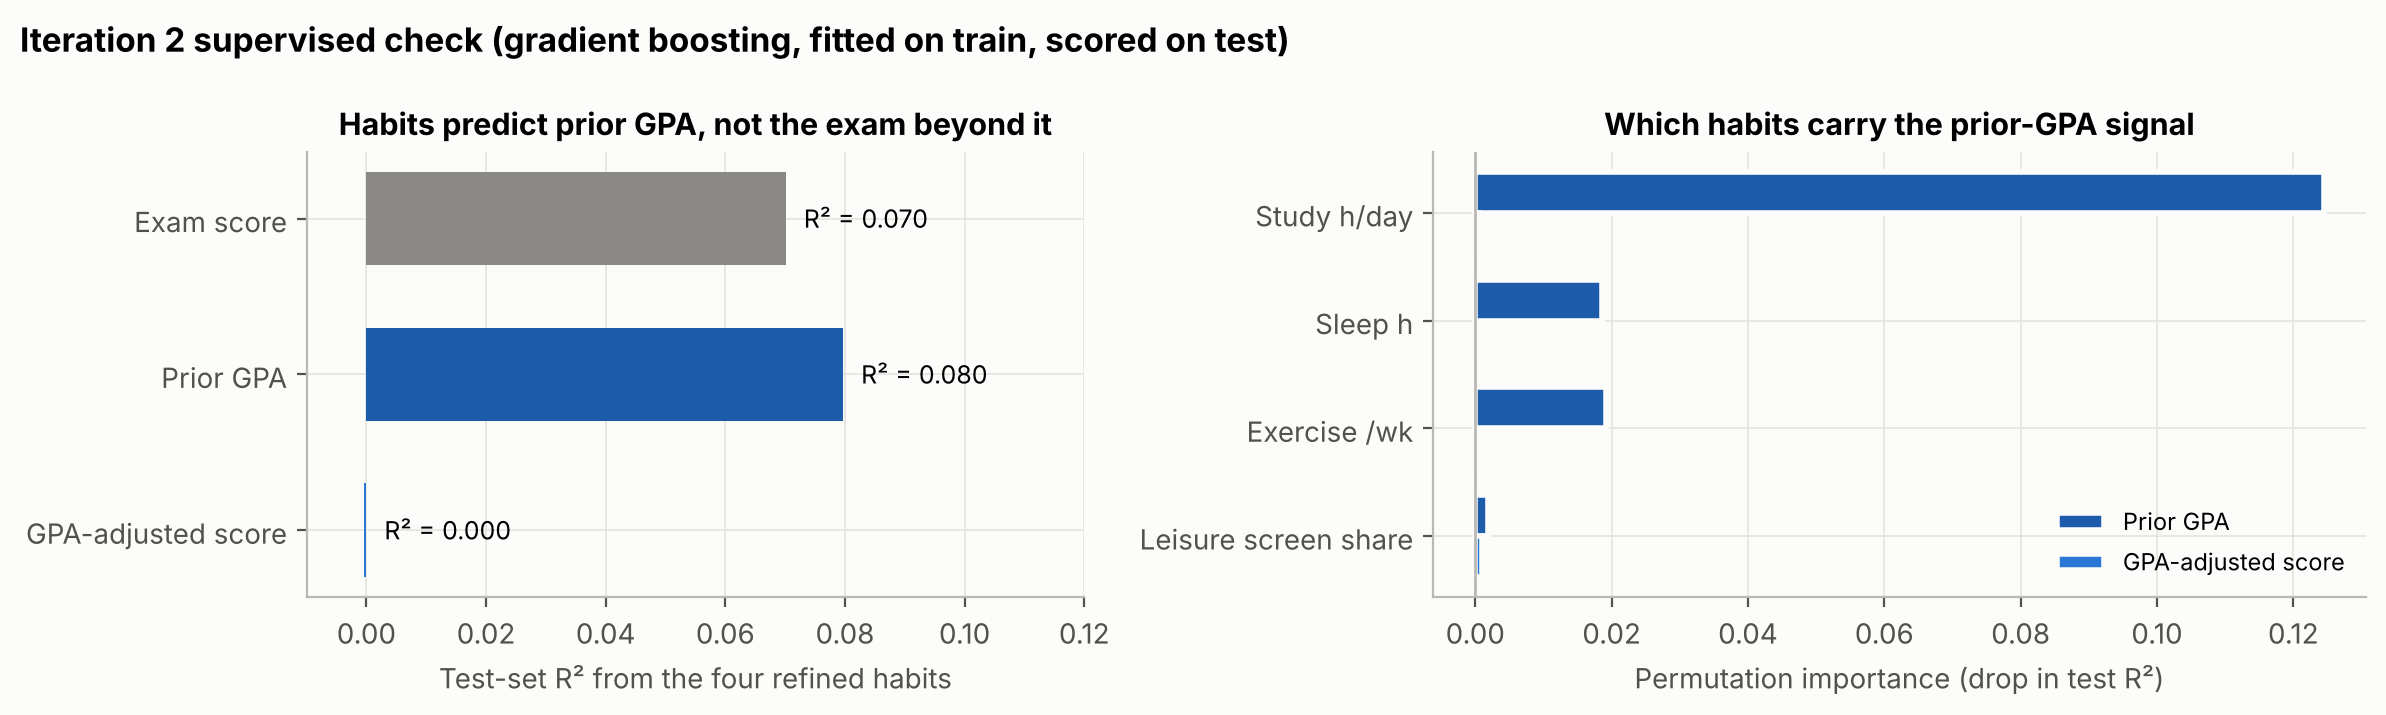
\includegraphics[width=\textwidth]{images/M1_fig10_supervised_check.png}
  \caption{Supervised check: gradient boosting fitted on the four refined
  habits (train) and scored on the test split. Habits explain $R^2=0.070$ of
  the exam score and 0.080 of prior GPA, but 0.000 of the GPA-adjusted score.
  Permutation importance shows study hours carries most of the prior-GPA
  signal; no habit carries any adjusted-score signal.}
  \label{fig:m1-sup}
\end{figure}

\paragraph{Knowledge K2.}
\begin{enumerate}
  \item \textbf{There is one stable habit profile split}, and it is about
        how students use screen time: study-focused versus leisure-heavy.
        Sleep and exercise do not form profiles of their own.
  \item \textbf{The profile's 4.2-point advantage is entirely its prior-GPA
        advantage.} Study-focused students arrive with a higher prior GPA; once
        GPA is held fixed, the gap is zero with a confidence interval narrower
        than $\pm0.13$ points, on unseen test data and with the ceiling group
        removed (Fig.~\ref{fig:m1-gap}).
  \item \textbf{Coarse bands hide confounding.} The Below-80 gap that survived
        banding in iteration~1 (Fig.~\ref{fig:m1-conf1}) is GPA variation
        inside the band (Fig.~\ref{fig:m1-band}). Any ``effect within the
        lowest band'' found with these four bands, including the one in A1
        (Appendix) Fig.~20, should be re-checked against the fine-grained adjustment.
  \item \textbf{Habits mark the trajectory, not the exam.} Habits predict prior
        GPA about as well as they predict the exam (Fig.~\ref{fig:m1-sup}).
        Prior GPA is measured before the exam and the habits are measured once,
        so this is a cross-sectional association: students with
        study-focused habits have been doing better for longer. The data cannot
        show that changing a habit would raise a score, and nothing in it
        suggests an exam-specific benefit.
\end{enumerate}

\paragraph{Reproducibility.} Running \texttt{preprocess\_a3.py} and then
\texttt{m1\_clustering\_workflow.py} (about one minute) regenerates every figure and number in this section. Cluster labels and the
adjusted score for all 80{,}000 students are saved for use in Tableau,
in \texttt{m1\_cluster\_assignments.csv.gz} under \texttt{Member1/outputs}.
